\documentclass{article}
    % General document formatting
    \usepackage[margin=0.7in]{geometry}
\usepackage[parfill]{parskip}
\usepackage[utf8]{inputenc}

% Related to math
\usepackage{amsmath,amssymb,amsfonts,amsthm}
\usepackage{graphicx}
\usepackage{enumitem}
\usepackage{tikz}
\usepackage{xcolor}
\usepackage{gensymb}
\setenumerate[1]{label=\thesubsection.\arabic*.}
\setenumerate[2]{label*=\arabic*.}


    % TODO: change thesis information
    \newcommand*{\getOrganisation}{Student Airrace}
    \newcommand*{\getTitle}{Technical Regulations}
    \newcommand*{\getAuthor}{Orga team}
    \newcommand*{\getDate}{12.01.2023}
    \newcommand*{\getVersion}{v0.0.1}
    \newcommand*{\getLocation}{Munich}


\begin{document}


\begin{titlepage}
    % HACK for two-sided documents: ignore binding correction for cover page.
    % Adapted from Markus Kohm's KOMA-Script titlepage=firstiscover handling.
    % See http://mirrors.ctan.org/macros/latex/contrib/koma-script/scrkernel-title.dtx,
    % \maketitle macro.
    \oddsidemargin=\evensidemargin\relax
    \textwidth=\dimexpr\paperwidth-2\evensidemargin-2in\relax
    \hsize=\textwidth\relax
  
    \centering
  
    \IfFileExists{logos/STAR_logo.png}{%
      
\includegraphics[height=20mm]{logos/STAR_logo.png}
    }{%
      \vspace*{20mm}
    }
  
    \vspace{5mm}
    {\huge\MakeUppercase{\getOrganisation{}}}\\
  
    \vspace{5mm}
  
    \vspace{20mm}
  
    \vspace{15mm}
    {\huge\bfseries \getTitle{}}
  
    \vspace{15mm}
    {\getDate{}}
    \vspace{10mm}
    \linebreak
    {\getVersion{}}
    \linebreak
    { \getLocation{}}
  
  
  
  
  
    \IfFileExists{logos/tum_logo.png}{%
    \vfill{}
    
\includegraphics[height=20mm]{logos/tum_logo.png}
      }{}
  \end{titlepage}

\tableofcontents{}
\newpage

{\bf Note: Contents marked in \textcolor{red}{red} are still subject to change and are to be seen as current estimations and placeholders.}

\section{Definitions}

\subsection{Propeller Disks}
\begin{enumerate}
  \item The propeller disk is a cylinder within the Body-Fixed-Frame that is defined by the full rotation of a single propeller. Each propeller has their own respective propeller disk. 
  \item The center axis of this cylinder, is reffered to as the propeller shaft. Its interesction with the very center of the disk will be used as a reference point for any measurements taken from the propeller disk. Every measurement which mentions the propeller disk within these regulations refers to this point.
\end{enumerate}


\subsection{Vehicle Coordinate Frame Definitions}
\begin{enumerate}
  \item The Ground Plane is defined as the ground when the aircraft is in landed position with the landing gear extended. Even during flight this plane stays fixed to the Body-Fixed-Frame of the aircraft.
  \item The XY-Plane is parallel to the ground plane. Its exact position is defined by the intersection with the lowest propeller disk center.
  \item X-Axis and Y-Axis
  \item The z-Axis is defined as an axis perpendicular to the xy-plane. It intersects the XY-plane in the aircrafts center of gravity. As usual in a Body-Fixed Aircraft frame the positive direction is pointin downwards in during landed state.
  \item The Coordinate frames must be clearly marked and made visible in the competitors technical report. 
\end{enumerate}

\subsection{Power Units}
\begin{enumerate}
  \item A power unit is defined as a lift-producing actuator and its associated control electronics. In a classical multicopter design, this would include a single electronic speed controller (ESC) on the aircraft, the motor it controls, and the propeller attached to the motor. Each of these components constitutes a single powertrain. 
  \item To ensure that only legitimate power units are used in the competition, all devices delcared as power units must strictly be used for producing thrust. Any components that are used for cooling or other purposes will not be considered as power units.
  \item The vehicle must be able to be able to safely continue a stable flight if any single power unit fails.  
\end{enumerate}



\section{Environmental Envelope}
\begin{enumerate}
  \item Teams will only be permitted to fly their aircraft if they meet the necessary operational conditions and requirements. These conditions must be fully satisfied before any flights may be conducted:
\begin {itemize}
  \item The aircraft must be able to operate in temperatures between \textcolor{red}{5 \degree C} and \textcolor{red}{30 \degree C}.
  \item The relative humidity must stay within \textcolor{red}{0\%} and \textcolor{red}{100\%}. 
  \item The aircraft must be able to operate within a range of air pressures, with a minimum of \textcolor{red}{950 hPa} and a maximum of \textcolor{red}{1050 hPa}.
  \item The average windspeed must stay below \textcolor{red}{6m/s}. Gusts may not be exceed \textcolor{red}{15m/s} within one hour before and during the flight.
  \item The aircraft must be designed and built to withstand flying in drizzle conditions, including maintaining stability and control and protecting sensitive equipment from moisture despite the presence of precipitation.
  
\end {itemize}
\end{enumerate}

\section{Aircraft Performance Requirements}

\subsection{Vehicle MTOW}
\begin{enumerate}
  \item The Maximum Weight of the vehicle during scruteneering must not exceed 22.5kg.
  \item The organizer will publish the weights of Equipement which must be used during the competition and thus added to the vehicle beforehand. Those weights wound count towards the maximum weight. 
  However the teams should plan their calculations for the vehicle with those weights added. The Maximum Takeoff Weight with this Equipement will not pass 25kg.  
  \item The Weight of the vehicle during scruteneering must at exceed \textcolor{red}{12kg}.  
\end{enumerate}

\subsection{Vehicle Thrust}
\begin{enumerate}
  \item The minimum Thrust measured on the vehicle Thrust Test Stand must exceed \textcolor{red}{300N} under standard atmospheric conditions.
  \item If the atmospheric conditions at the time of testing do not meet the ICAO standard atmosphere conditions, a correction factor based on the current air density will be applied to the thrust stand results in a linear manner.
\end{enumerate}


\section{Electronics}


\subsection{Power Source}
\begin{enumerate}
  \item The aircrafts power source must be electric. All motors and acutators on the aircraft must also be electrically driven.
  \item Vehicles powerd by combustion engines, \textcolor{red}{Hydrogen Cells or comparable fuel burning devices} are not permitted. 
\end{enumerate}

\subsection{Onboard Electronics}
\begin{enumerate}
  \item The maximum DC voltage across any two electrical connections on the aircraft must not exceed 60V.
  \item Team participants are permitted to use various battery types on their drones, provided that the batteries are compliant with EASA regulations for Unmanned Aerial Vehicles (UAV) and do not present a significantly elevated level of risk when compared to the use of a Lithium Polymer (Lipo) battery. 
  \item A fuse with a suitable current rating must be added in series with each battery in the propulsion system. 
  This fuse must be installed in-line with the positive terminal of the battery. Its maximum continuous current rating must be equal to or less than the maximum continuous discharge rating of the battery \textcolor{red}{times a safety factor of 1.3}. This helps to protect the battery, the propulsion system, and the aircraft as a whole from damage or failure due to overcurrent conditions.
  \item The flight control system must be fed by at least two differrent power sources. 
\end{enumerate}



\section{Aircraft Geometry}

\subsection{Vehicle Configurations}
\begin{enumerate}
  \item The vehicle must be able to takeoff and land vertically without posing as a safety hazard or showing drift.  
\end{enumerate}

\subsection{Powerunit Posititons}
\begin{enumerate}
  \item The aircraft used in the event must not have more than 16 power units. Any aircraft found to have more than this maximum will be disqualified from the competition.
  \item The rotor disks can be offset to each other however the teams prefer within the XY-plane. 
  \item The lowest point of a rotor disk may not be lower than 150mm above the ground when the aicraft is in landed state with the landing gear extended.
  \item The lowest point of a rotor disk may not be lower than 70mm above the ground when the aircraft is landed state without the landing gear extended (as might happen in a landing gear extension failure).
  \item The futhest distance between two main-motor-shafts in x direction divided by the furthest distance between two main-motor-shafts in y direction must lie between 0.5 and 2. 
  \item The rotor disks may be offset to each other in the z direction up until a maximum difference of +-400mm.
  \item The rotor disks may overlap when viewed in the xy-plane if a necessary seperation between the rotors during full-thrust with a safety factor of 3 or more at the closest position is ensured. If the distance between both disks exceeds at least 1/4 of the propeller diameter no prove is necessary, prove for must be provided by the teams in their safety report. 
  \item Rotors whichs rotor disks overlap or mesh within each other are not permitted. Even if mechanically or electronically coupled.
  \item The total vehicle size, including propellers, must not exceed a box with the side lengths of $x=3000mm$, $y=3000mm$, $y=1200mm$
  \item The total vehicle size, including propellers, must exceed a box with the side lengths of $x=1200mm$, $y=1200mm$, $y=300mm$
\end{enumerate}

\subsection{Powerunit Orientation}
\begin{enumerate}
  \item The motor angle in relation to the vehicles body frame must stay fixed at all times during flight. 
  \item All motors used may be individually tilted by a maximum of XX\degree  parallel to the X-Axis of the vehicles body system.
  \item All motors used may be individually tilted by a maximum of XX\degree  parallel to the Y-Axis of the vehicles body system.
  \item The teams may use spacers to quickly adjust these values to achieve different flight dyanmics.
  \item While the vehicle is standing on the ground, the lowest part of each propeller disk must have a ground clearence of at least 10cm. 
  \item The distance between the centers of the two motor centers the furthest from each other must exceed a direct distance of 1.20m and may not exceed a direct distance of 2.00m. 
\end{enumerate}


\subsection{Propeller Dimension}
\begin{enumerate}
  \item The minimum propeller diameter used on the main-motors must exceed $y=600mm$.
  \item The maximum propeller diameter used on the main-motors must not exceed $y=1200mm$.
  \item If varying propeller diameters are used on the main-motors the quotient must be within 0.67-1.5.
  \item \emph{Maximum Pitch settings etc?}
\end{enumerate}





\section{Aircraft Subsystems}

\subsection{Internal Cooling}
\begin{enumerate}
  \item Fans with a maximum diameter of 50mm are allowed to be fitted anywhere on the vehicle. These do not count as rotors and thus do not need to follow the orientation rule from earlier.
  \item Water cooling is permitted. 
\end{enumerate}

\subsection{AI onboard computer}
These rules only apply if the competitor decides to participate in the autonomy discipline. 
\begin{enumerate}
  \item Every computation, that directly influences the trajectory of the aircraft must be executed onboard.
  \item The companion computer must be equipped with enough storage, so that decisions made by the autonomy stack can be analysed afterwards in case of a failure. 
  \item The navigation and trajectory planning algorithms must be validated in a Hardware in the loop(HITL) simulation before the race starts, to make sure that the code works and the computer is capable to process the workloads.
  \item A malfunction in the autonomy stack must result in a position hold state. 
  \item Every sensor that perceives the environment must be onboard.
\end{enumerate}


\section{Groundstation}
\subsection{Video Transmission}
\begin{enumerate}
  \item The teams must use a digital video connection suitable for flying a aircraft at the competition.  
  \item The video transmission method must be legal to use in Germany. This includes mainly following the officially allowed frequencies and power outputs and having a valid CE certificate for the video system.
\end{enumerate}

\subsection{External Cooling and Heating}
\begin{enumerate}
  \item Teams may use leafblowers or comparable devices to externally cool their aircraft after a flight. However they aircraft must but not by live anymore and shut down, shunt plug disconnected.  
  \item Teams may preheat their batteries to an optimum operating temperature with external tools such as heating boxes or heating blankets.
\end{enumerate}

\section{Standardized Parts}

\subsection{T-Camera-Pod}
\begin{enumerate}
  \item The teams will be provided with a standardized camera and sensor housing which goes on top of the UAS.
  \item \emph{What kind of mounting plate/adapter does this need?}
  \item \emph{Do we supply the teams only with a mockup and specifications attach the actual camera in the final competition?}
  \item \emph{What FOV does the camera need? How do we define the exact position?}
\end{enumerate}



\subsection{Avionics suite}
\begin{enumerate}
  \item \emph{How big and heavy does the avionics suite need to be?}
  \item \emph{Which kinds of instruments/sensors do we put in there?}
  \item \emph{Should we attach some sort of safety shut off switch into this avionics box?}
  \item \emph{Will this box be connected to the T-Wing or exist on it's own?}
  \item \emph{Where do we put this avionics box?}
\end{enumerate}

\subsection{Mounting Adapter Dimensions}
In the Thrust Stand Event, competitors are required to provide their own adapter for attaching their drone to the Thrust Test Stand. The interface provided by the event organizer is standardized and shall be refered to as the Lower Mounting Plate. The Lower Mounting Plate is the standardized interface, provided by the Organizer, to which the teams must attach their drone via the Upper Mounting Plate. The Upper Mounting Plate is the part of the interface that teams need to design and develop as a part of their competition drone. Teams must ensure that their drone's upper mounting plate is compatible with the standard Lower Mounting Plate, and that the drone can be securely attached to the test stand. 
\begin{figure}
  \centering
   \IfFileExists{figures/FullThrustStand3D.jpg}{%
   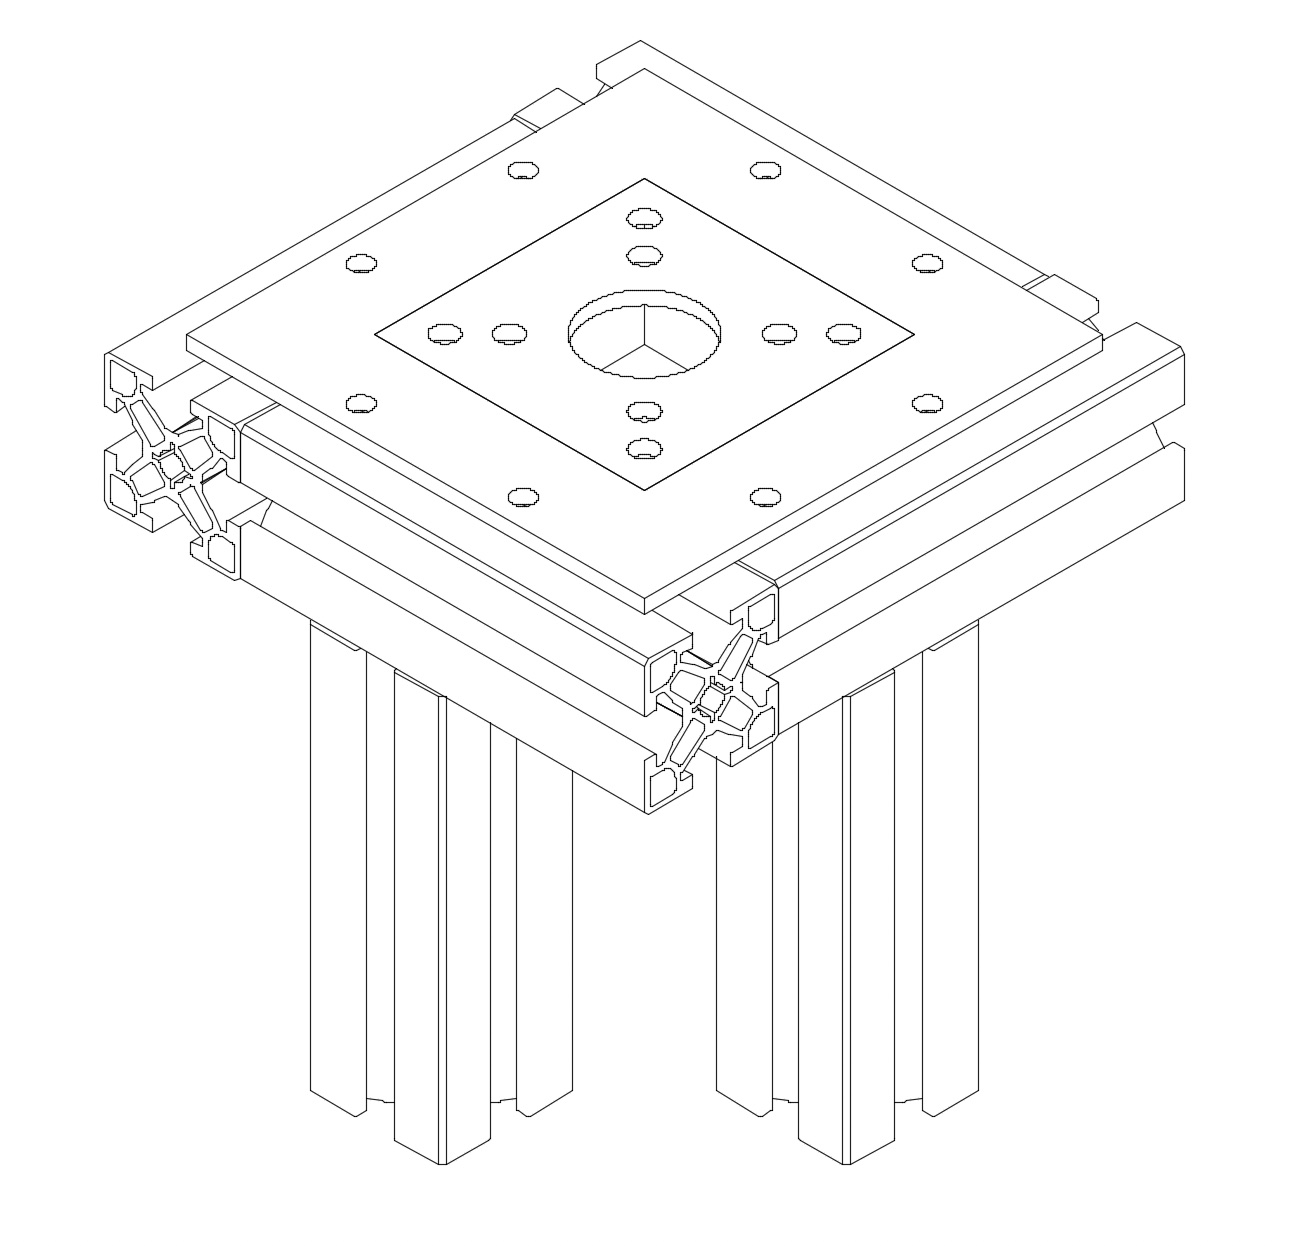
\includegraphics[height=50mm]{figures/FullThrustStand3D.jpg}
   }{%
   \vspace*{50mm}
   }
 \caption{\textit{Isometric view of the Thrust Stand Adapter with the standardized Lower Mounting Plate, as provided by the organizer. The competitor's Upper Mounting Plate, which is responsible for attaching their drone to the adapter, is not depicted in the photo. Note that the design and dimensions of the Thrust Stand Plate are subject to change, but the interface for attachment, the Lower Mounting Plate, will remain unchanged.}}
 \end{figure}

\begin{enumerate}
  \item The XY-plane of the drone must be parallel to the bottom surface of the Upper Mounting Plate. Additionally, the bottom of the Upper Mounting Plate may not be positioned closer than 250mm to the center of gravity of the drone in the Z-direction.  
  \item The upper mounting plate must have four through-holes with a diameter of 9mm. They must be arranged in a 2 by 2 pattern. The teams have the opportunity to choose between two different sets of though-holes:
    \begin{itemize}
      \item Smaller Set A: Four 9mm holes with a distance of ${\Delta}x=50mm$ and ${\Delta}y=50mm$.
      \item Bigger Set B: Four 9mm holes with a distance of ${\Delta}x=74mm$ and ${\Delta}y=74mm$.
    \end{itemize}
  \item The competitors flange can not exceed the volume above the mounting plate within 200mm above the bottom of the upper mounting plate. 
  \item The design of the Upper Mounting Plate must include sufficient clearance on the top surface to allow for the placement of M8 Screws and M8 washers, in accordance with ISO 7089 standards, through the holes. The Student AirRace organizers will ensure that these screws can be securely fastened on the opposite side using locknuts.
  \item The upper mounting plate and further structural mounts which only facilitate the attachment of this holding plate to the test stand may be removed by the teams for the flights. 
  \item The drone must be designed and built to transfer all of its thrust through the Upper Mounting Plate and its associated screws. Within the safety report the teams must provide calculations demonstrating that their adapter is capable of transferring the expected loads with a minimum safety factor of 5. \end{enumerate}

\begin{figure}
  \centering
  \IfFileExists{figures/ThrustStandTeamAdapterTechnicalDrawing.jpg}{%
  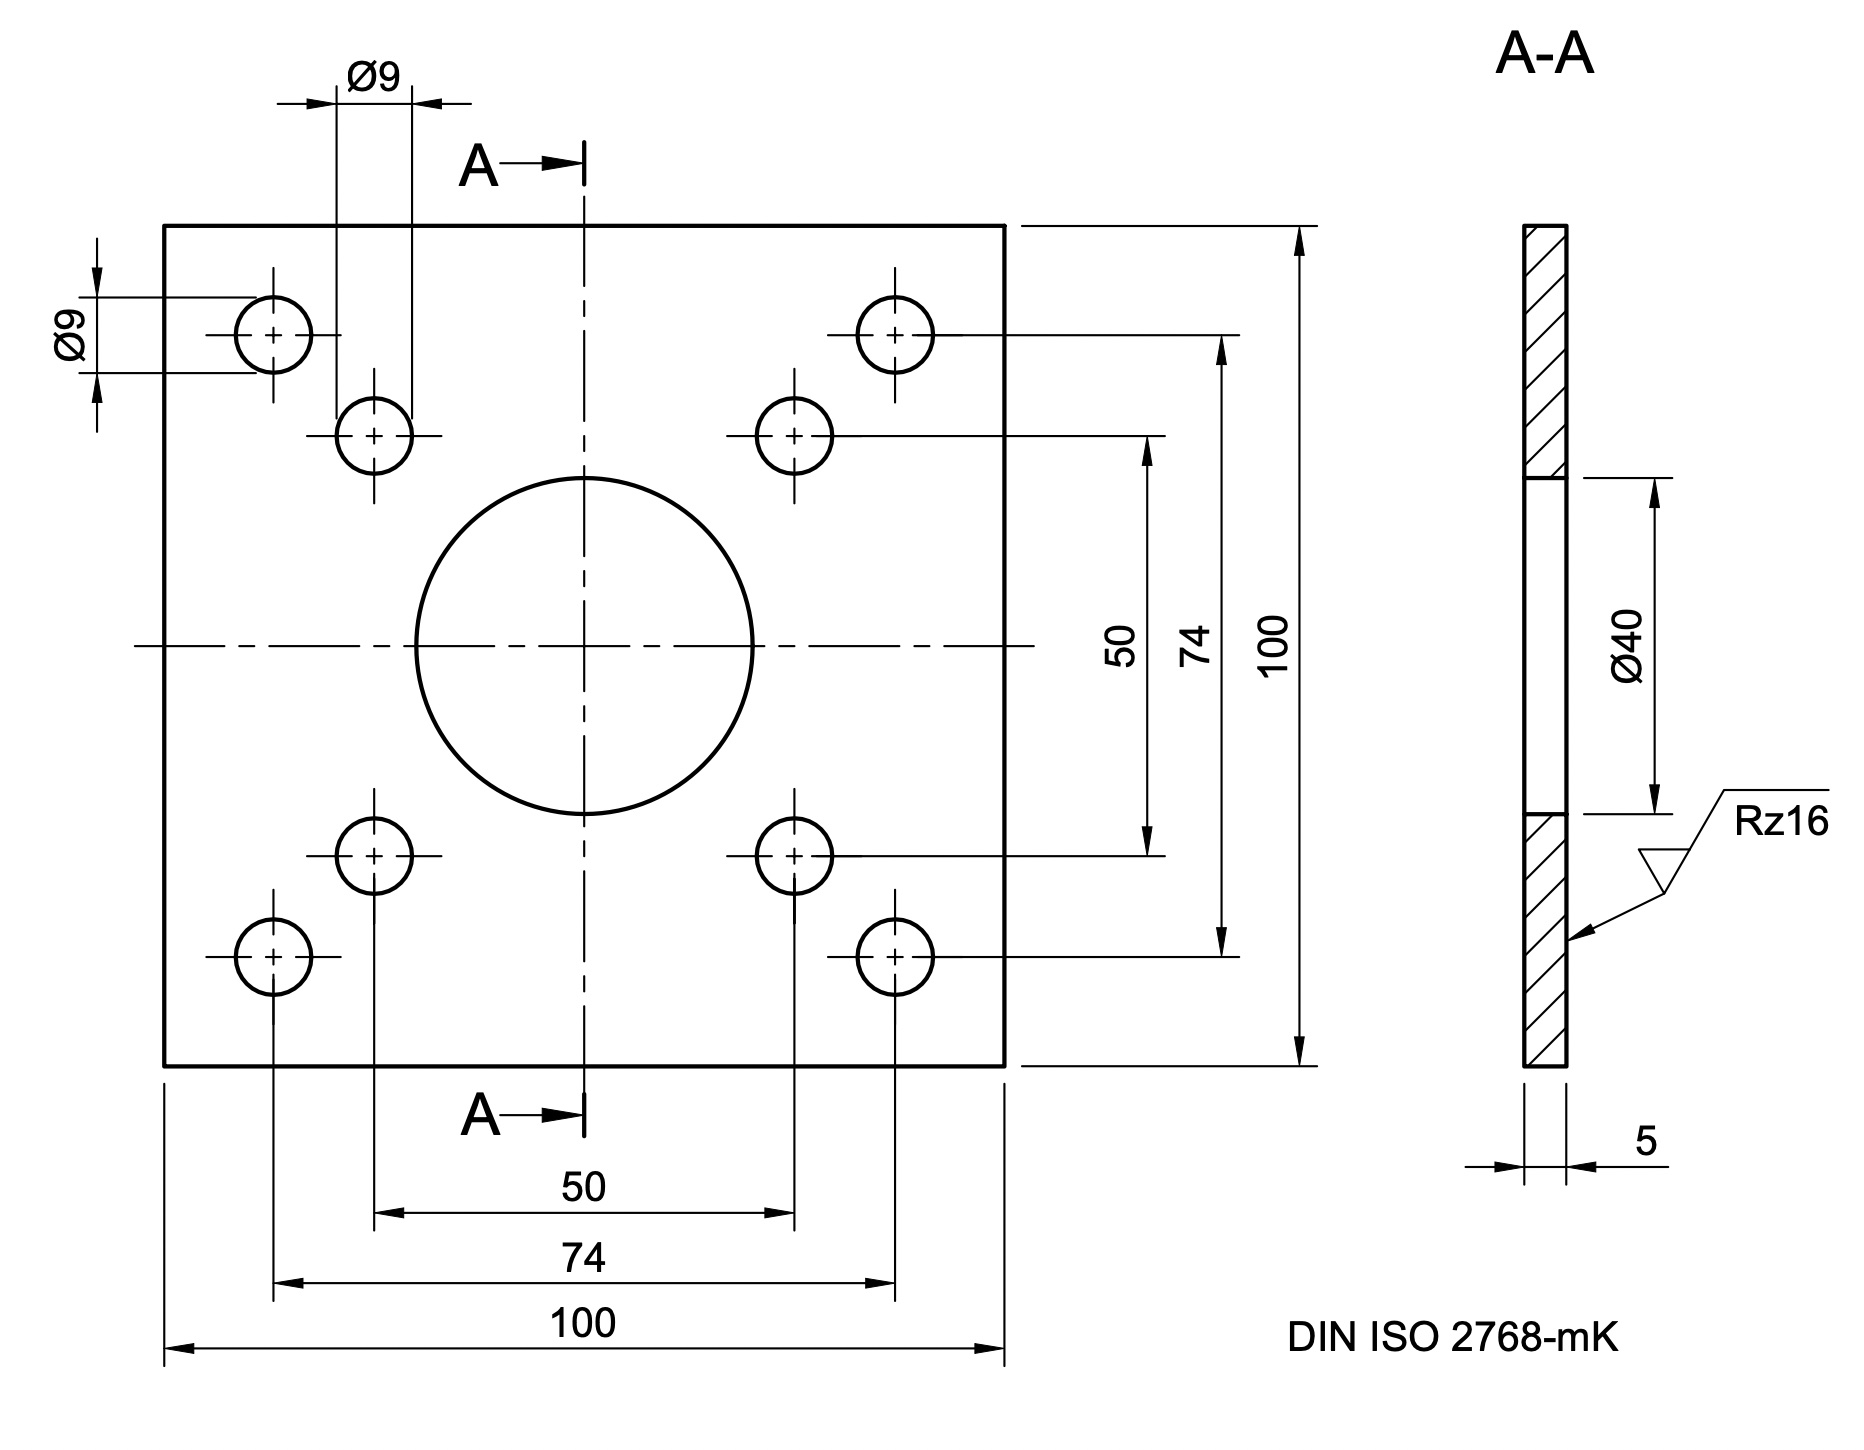
\includegraphics[height=100mm]{figures/ThrustStandTeamAdapterTechnicalDrawing.jpg}
  }{%
  \vspace*{100mm}
  }
\caption{\textit{Technical Drawing of the Lower Mounting Plate provided by the Organizer. Attention: The Adapter shown here is only the inner part of the full plate which will be at the competition. The sidelengths will ne bigger than 100mm. You cannot exceed the side lengths of 100mm.}}
\end{figure}

\begin{figure}
 \centering
  \IfFileExists{figures/ThrustStandTeamAdapter3D.jpg}{%
  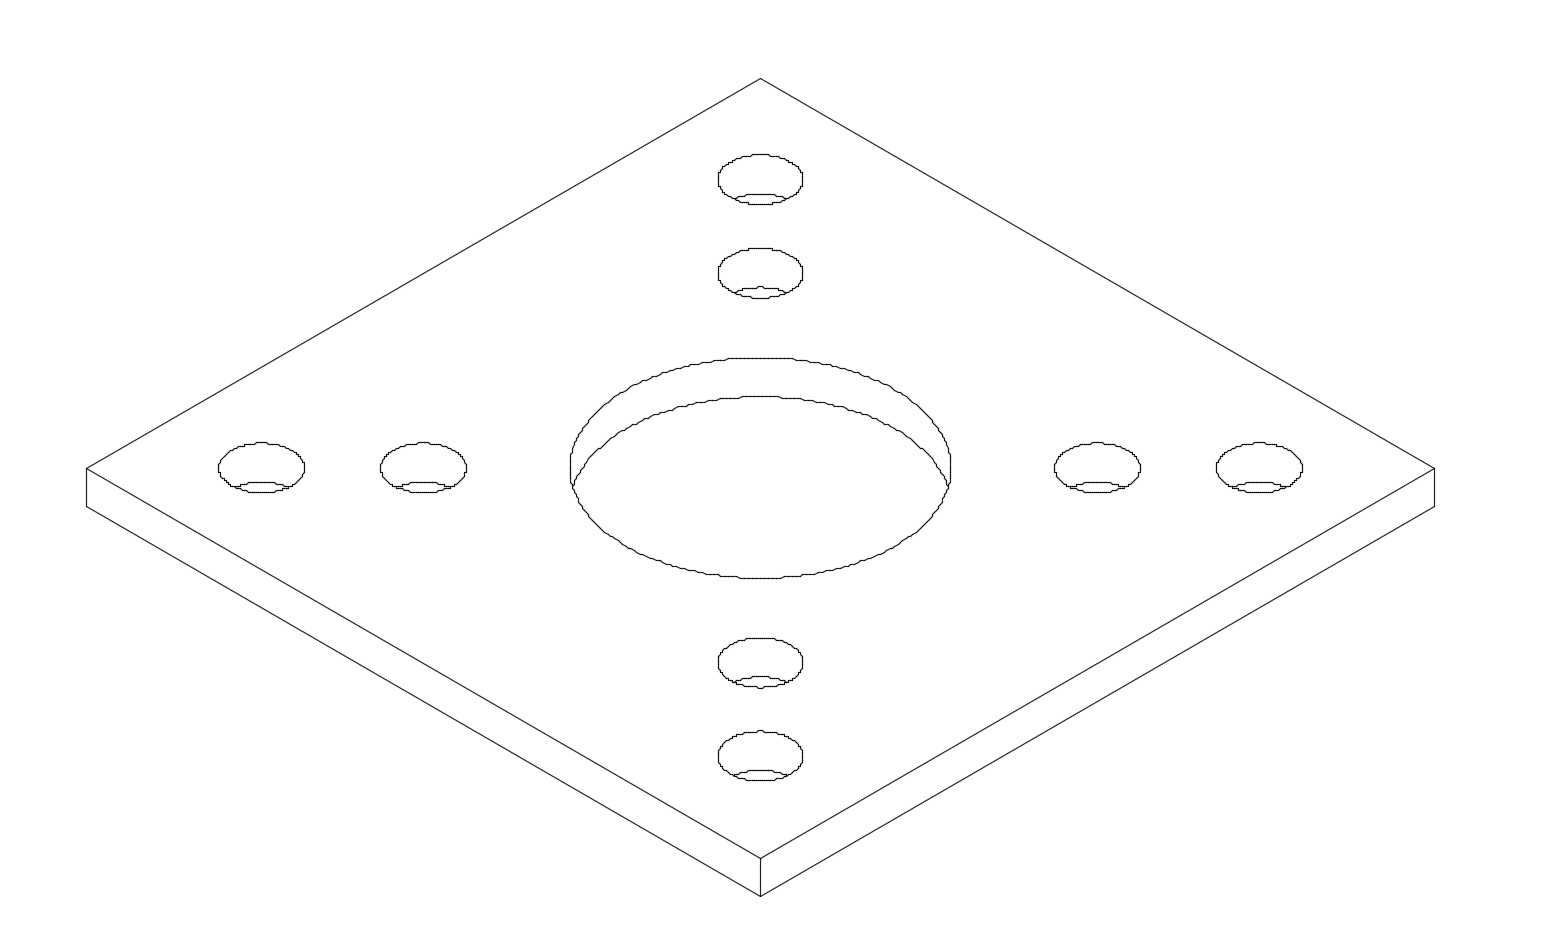
\includegraphics[height=50mm]{figures/ThrustStandTeamAdapter3D.jpg}
  }{%
  \vspace*{50mm}
  }
\caption{\textit{Isometric view of the Thruststand-Adapter.}}
\end{figure}



\subsection{Timing Equipement}
\begin{enumerate}
  \item The organizer will be responsible for measuring the race time using external optical systems such as cameras. Teams will not be required to install any timing sensors or equipment within their drone. The organizer will provide and operate the necessary timing equipment.
\end{enumerate}

\section{Safety Systems}

\subsection{Shunt Plug}
The Shunt Plug serves as a manual and physical means for disarming the aircraft. It is supposed to completly disconnect the battery power from the motors and be able to be removed by hand in case of an emergency.
\begin{enumerate}
  \item A Shunt Plug must be wired between the leads of the battery system and the electronic speed controllers (or Power Distribution Device) for manual disarming and arming of the aircraft's power system.
  \item The Shunt Plug must be removable with one hand and without any tool.
  \item Installing a physical switch mounted on the drone is not permitted and will not be considered a valid Shunt Plug.
  \end{enumerate}
  
  
  

\subsection{Ground Emergency Switch}
\begin{enumerate}
  \item Teams need to at least have a special kill switch programmed to their Transmitter or console from which they control the aircraft. This kill switch needs to shut down all flight controller motor outputs. 
  \item An arm/disarm switch is not sufficient as a kill switch.
  \item The aircraft needs to be equipped with a Land function which autonomously lands the aircraft at the current position. A switch needs to be bound on the Transmitter/Ground Station from which the team controls the aircraft from.  
  \item \emph{Which Devices will be supported by the organizers? Which do the teams need to buy?}
  \item \emph{Where do the teams have to put the emergency shut down devices?}
  \item \emph{Do the devices operate relays or shut downn via MAVLINK?}
\end{enumerate}


\subsection{Remote Emergency System}
The organizer reserves the right to implement a remote emergency shutdown system within the avionics blackbox of the aircraft. However, it is unlikely that the development of this device will be completed prior to the first competition. Therefore, it is especially important for teams to equip their aircraft with multiple redundant methods of turning off their aircraft in the event of an emergency or loss of control.

\section{Safety Requirements}
Given that the competition is already set up in a manner compliant with legal regulations for drone operations, it may be difficult to establish specific and quantitative safety regulations. However, the organizer has still implemented certain guidelines to ensure the safety of all participants. We strongly encourage teams to make every effort to follow these guidelines as closely as possible to ensure the safety of all those involved in the competition. 
\\ \\ 
However is important to note that safety processes, such as this one, are often qualitative in nature. The organizer will strive to ensure that the safety guidelines are applied in a consistent and fair manner for all competitors, using EASA SORA process as a guideline as much as possible, as it will positively impact the safety report. The organizer will take the necessary steps to review and evaluate the safety of each drone individually. All teams will be treated in the same way, with the same degree of scrutiny and attention to detail, to ensure a safe and fair competition.

\begin{enumerate}
  \item The design and construction of the drone must not include any single points of failure that would result in a crash with catastrophic outcome. Teams must demonstrate through design calculations, simulations, and testing that the drone can safely operate even in the event of a failure. Any drone that is deemed to have a single point of failure that would lead to a crash with catastrophic outcome will not be permitted to compete. \\ \\
  The rule for no single cause for failure shall include specifically the following points:
    \begin{itemize}
      \item Lift provided by the motors
      \item Power systems
      \item Emergency modes
      \item Video signal
      \item Transmitter/Control signal
      \item Fly Away Protection 
    \end{itemize}
  It is also worth noting that this list is not exhaustive and teams should consider other possible failure points for their drone design.
  \item It is recognized that eliminating all single points of failure that could lead to a crash with catastrophic outcome may not be feasible due to cost constraints. However, teams are expected to have implemented multiple safety systems in their drone design to minimize the risk of harm to individuals on the ground. Additionally, the organizer will have safety measures in place to help mitigate risk during the event.
  \item Teams are required to use state-of-the-art or advanced technology in the design and construction of their drone.
  \item Where applicable and possible, teams are encouraged to use standards and norms in the design and construction of their drone. Adhering to standards and norms such as those established by EASA, EUROCAE or ARP documents etc. can have a positive impact on the safety report. Teams should reference any standards and norms used in their design in the safety report.
  \item Any attempts to circumvent or subvert the safety regulations put in place for the competition will not be tolerated. Such efforts include, but are not limited to, attempting to bypass safety checks, falsifying safety reports, and using non-compliant equipment. Any team found to be in violation of these regulations will be immediately disqualified from the competition without exception, and may face further consequences as deemed appropriate by the organizer.
  \item The Organizers strongly recommend that teams adhere to the processes established within the EASA SORA (Specific Operations Risk Assessment) process outlined in the EU ordinance 2019/947. Compliance with this process can aid teams in identifying and mitigating safety risks associated with their drone operation, and demonstrate to the Organizers a commitment to safety. Adherence to SORA is not mandatory, but following it will positively impact the safety report.
\end{enumerate}


\section{Regulatory Requirements}
\begin{enumerate}
  \item The aircrafts themselves as well as their operation, must be certifiable within the EASA A3 class in Germany. To fall within this class a selfbuild aircraft, must follow rules which are set out by the authorities. 
  The following points include some of them yet not include all information necessary. Competitors will need to do their own research and make sure to keep up to date with the regulatory requirement on their own:
  \item Analog video signals are only allowed on certain frequency channels between 5725MHz and 5875MHz, and must not exceed an equivalent isotropically radiated power (EIRP) of 25mW.
  \item All RC transmitters must be equipped with an EU-LBT option and must hold a CE certification. Teams must carry a declaration of conformity to this certification and present it to the organizers at the competition.
  \item In order to ensure compliance with regulatory standards, all other radio transmitters including radio, telemetry, and video transmitters must hold a CE certification. Teams must be prepared to present the declaration of conformity for these certifications upon request by the organizers.
  \item The maximum takeoff weight (MTOW) for the aircraft must not exceed 25kg.
  \item While pilots are required to fly the aircraft within line of sight, they may use a screen or FPV goggles as long as a secondary spotter is present to assist them.
  \item It is mandatory for all drones to have a commercial drone insurance policy with a minimum coverage of 750,000 SDZ.
  \item The aircraft must be registered with EASA or in Germany and must have an e-ID.
  \item The aircraft must also have a fireproof badge displaying the EASA e-ID of the vehicle operator.
  \item In order to participate, pilots must hold a valid EASA A1/A3 license and be at least 16 years of age.
\end{enumerate}

\section{Additional Requirements}
\begin{enumerate}
  \item It is required that flightbooks and flight documentation are completed and maintained for each flight, to accurately record and track the flight hours and experiences of the pilots and aircraft.
  \item In order to ensure the safety and regulatory compliance of the competition, standard and emergency checklists, as well as an emergency response plan, must be in place and followed for every flight.
  \item Prior to takeoff, pilots must gather and review relevant NOTAMs, airspace information, and weather conditions to ensure the planned flight can be safely conducted.
  \item After being accepted into the competition the teams will be provided with a specialized weather forecasting and analysis tool. This tool was developed specifically for use in professional aviation by one of the competitions partners. 
  This tool will allow the teams to accurately assess and predict the weather conditions which they will encounter during their testflights and development, helping to ensure the safety and success of their operations. 
  \item All electronic off-the-shelf components used in the competition, must be CE certified to ensure they meet necessary safety and performance standards.
  \item The competition teams are expected to foster a "just culture" within their organization, promoting the reporting of incidents and a focus on safety. \textcolor{red}{Student AirRace is also seeking to provide the teams with workshops about this topic.}
  \item Following each flight, a report must be written by the team, detailing any issues or concerns that arose during the flight. It can optionally be sumitted to the organizer to give them feedback on their rules and the teams current process.
\end{enumerate}







\end{document}